
%%%%%%%%%%%%%%%%%%%%%%%%%%%%%%%%%%%%%%
\documentclass{article}
\usepackage{Sweave}
\usepackage{graphicx}
\usepackage{tabularx}
\usepackage{hyperref}
\usepackage{natbib}
\usepackage{pdflscape}
\usepackage{array}
\usepackage{gensymb}
\usepackage{amsmath}
\usepackage{longtable}
\usepackage{xr}
\usepackage[small]{caption}

\setkeys{Gin}{width=0.8\textwidth}
\setlength{\captionmargin}{30pt}
\setlength{\abovecaptionskip}{10pt}
\setlength{\belowcaptionskip}{10pt}
 \topmargin -1.5cm        
 \oddsidemargin -0.04cm   
 \evensidemargin -0.04cm
 \textwidth 16.59cm
 \textheight 21.94cm 
 \parskip 7.2pt          
 \parindent 0pt
\usepackage{setspace}
\externaldocument{/Users/aileneettinger/Documents/GitHub/ospree/docs/budburst/budburstms}
\externaldocument{/Users/aileneettinger/Documents/GitHub/ospree/docs/budburst/budburst_supp}
%%%%%%%%%%%%%%%%%%%%%%%%%%%%%%%%%%%%%%

\begin{document}

\bibliographystyle{..//..//refs/bibstyles/naturemag}
\title{Extended Data:  Winter temperatures predominate in spring phenological responses to warming} 

\author{A. K. Ettinger, C. J. Chamberlain, I. Morales-Castilla, D. M. Buonaiuto, D. F. B. Flynn, \\ T. Savas, J. A. Samaha \& E. M. Wolkovich}
\date{} 
\maketitle  
%%%%%%%%%%%%%%%%%%%%%%%%%%%%%%%%%%%%%%%%%%%%%%%%%%%
\renewcommand{\thefigure}{ED\arabic{figure}}


\begin{figure}[h!]
\centering
\noindent 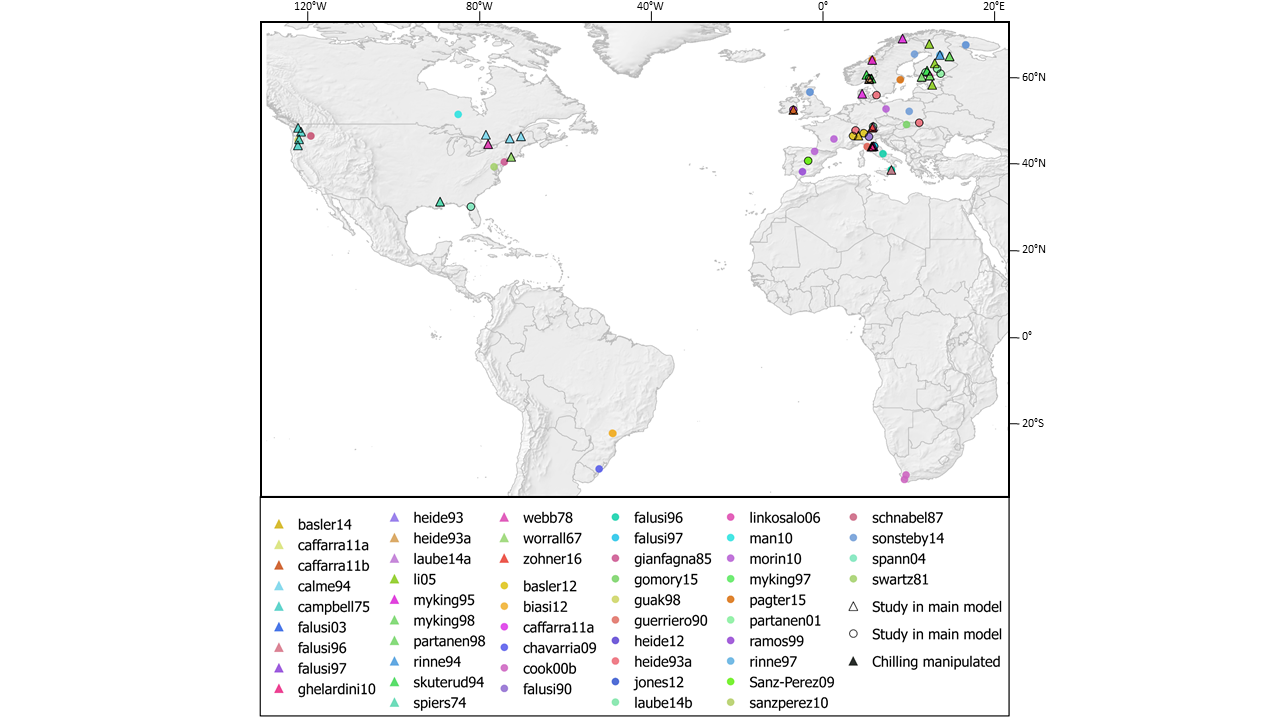
\includegraphics[width=0.9\textwidth]{..//..//analyses/bb_analysis/figures/EDFig1_OSPREECOORDSwcoords.png}
\caption{\textbf{Map of days to budburst experiments in the OSPREE database.} Legend shows each dataset included in the main OSPREE model with all species and treatments (Tables \ref{tab:modsz}, \ref{tab:modsnonz}); symbols outlined in black represent datasets for which chilling was manipulated experimentally or through multiple field sample dates. See Table \ref{tab:ref} for the reference associated with each dataset.}
\label{fig:map}
\end{figure}


\begin{figure}[h!]
\centering
\noindent 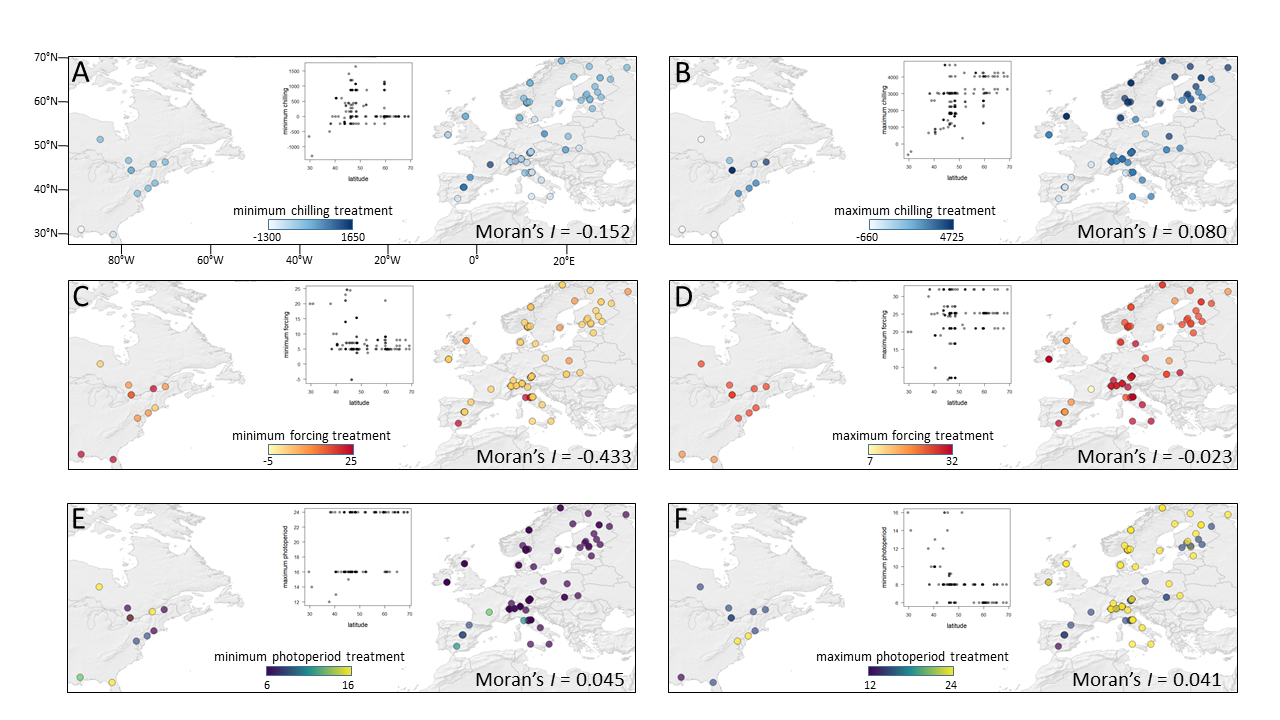
\includegraphics[width=0.9\textwidth]{..//..//analyses/bb_analysis/figures/EDFig2_minmaxtreatments_COORDS.png}
\caption{\textbf{Map of maximum and minimum chilling, forcing, and photoperiod treatments}, across all data included in our main model, and the locations where each experiment was conducted. We did not find strong positive spatial autocorrelation---\emph{i.e.}, indicating higher similarity in the treatments applied to experiments in nearby locations---in either minimum (A,C,E) or maximum (B,D,F) treatments, as measured by Moran's \emph{I} (shown above for European sites). Insets show relationship of each cue's treatment level with the latitude of the experiment.}
\label{fig:trtmap}
\end{figure}

\newpage
\begin{figure}[h!]
\centering
\noindent 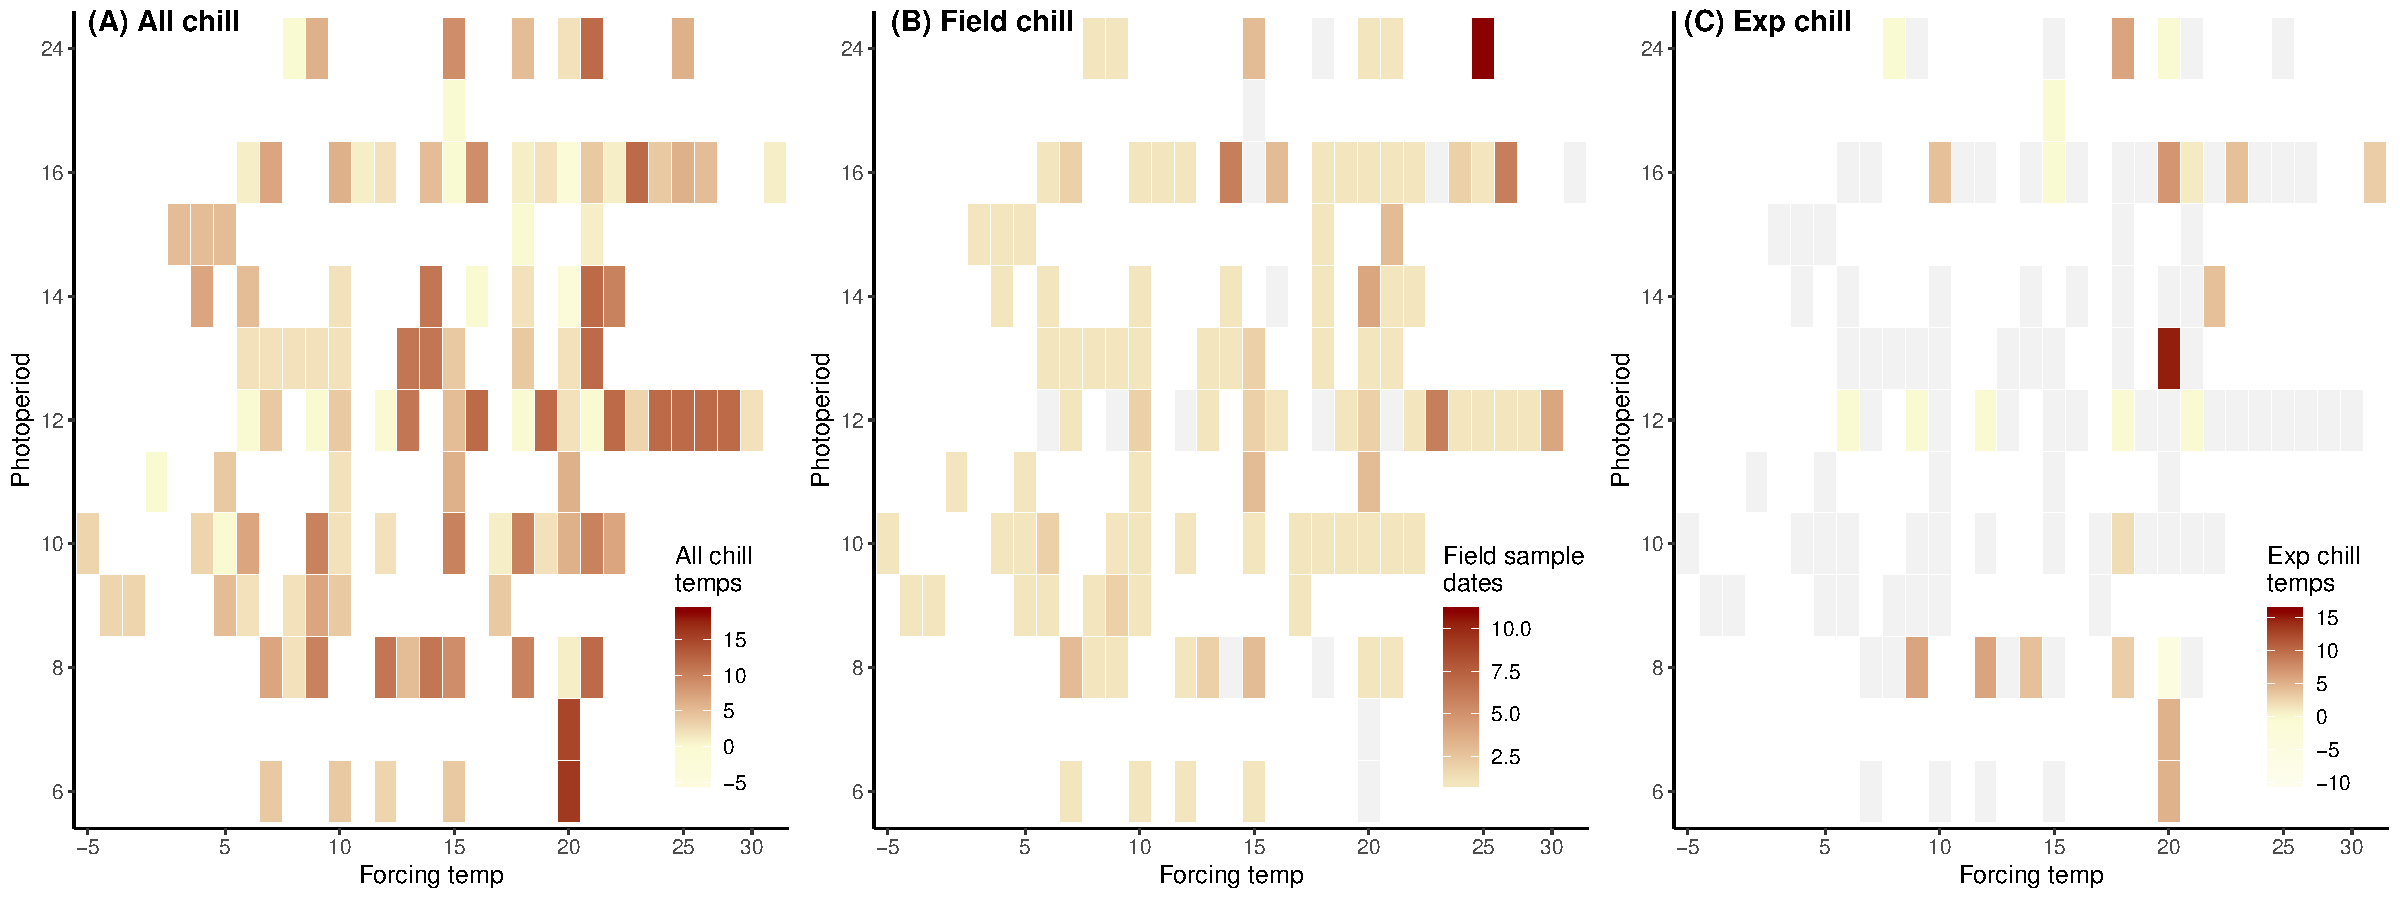
\includegraphics[width=0.9\textwidth]{..//..//analyses/bb_analysis/figures/studydesign/EDFig3_studydesign_heat3panelallsppmodel.pdf}
\noindent 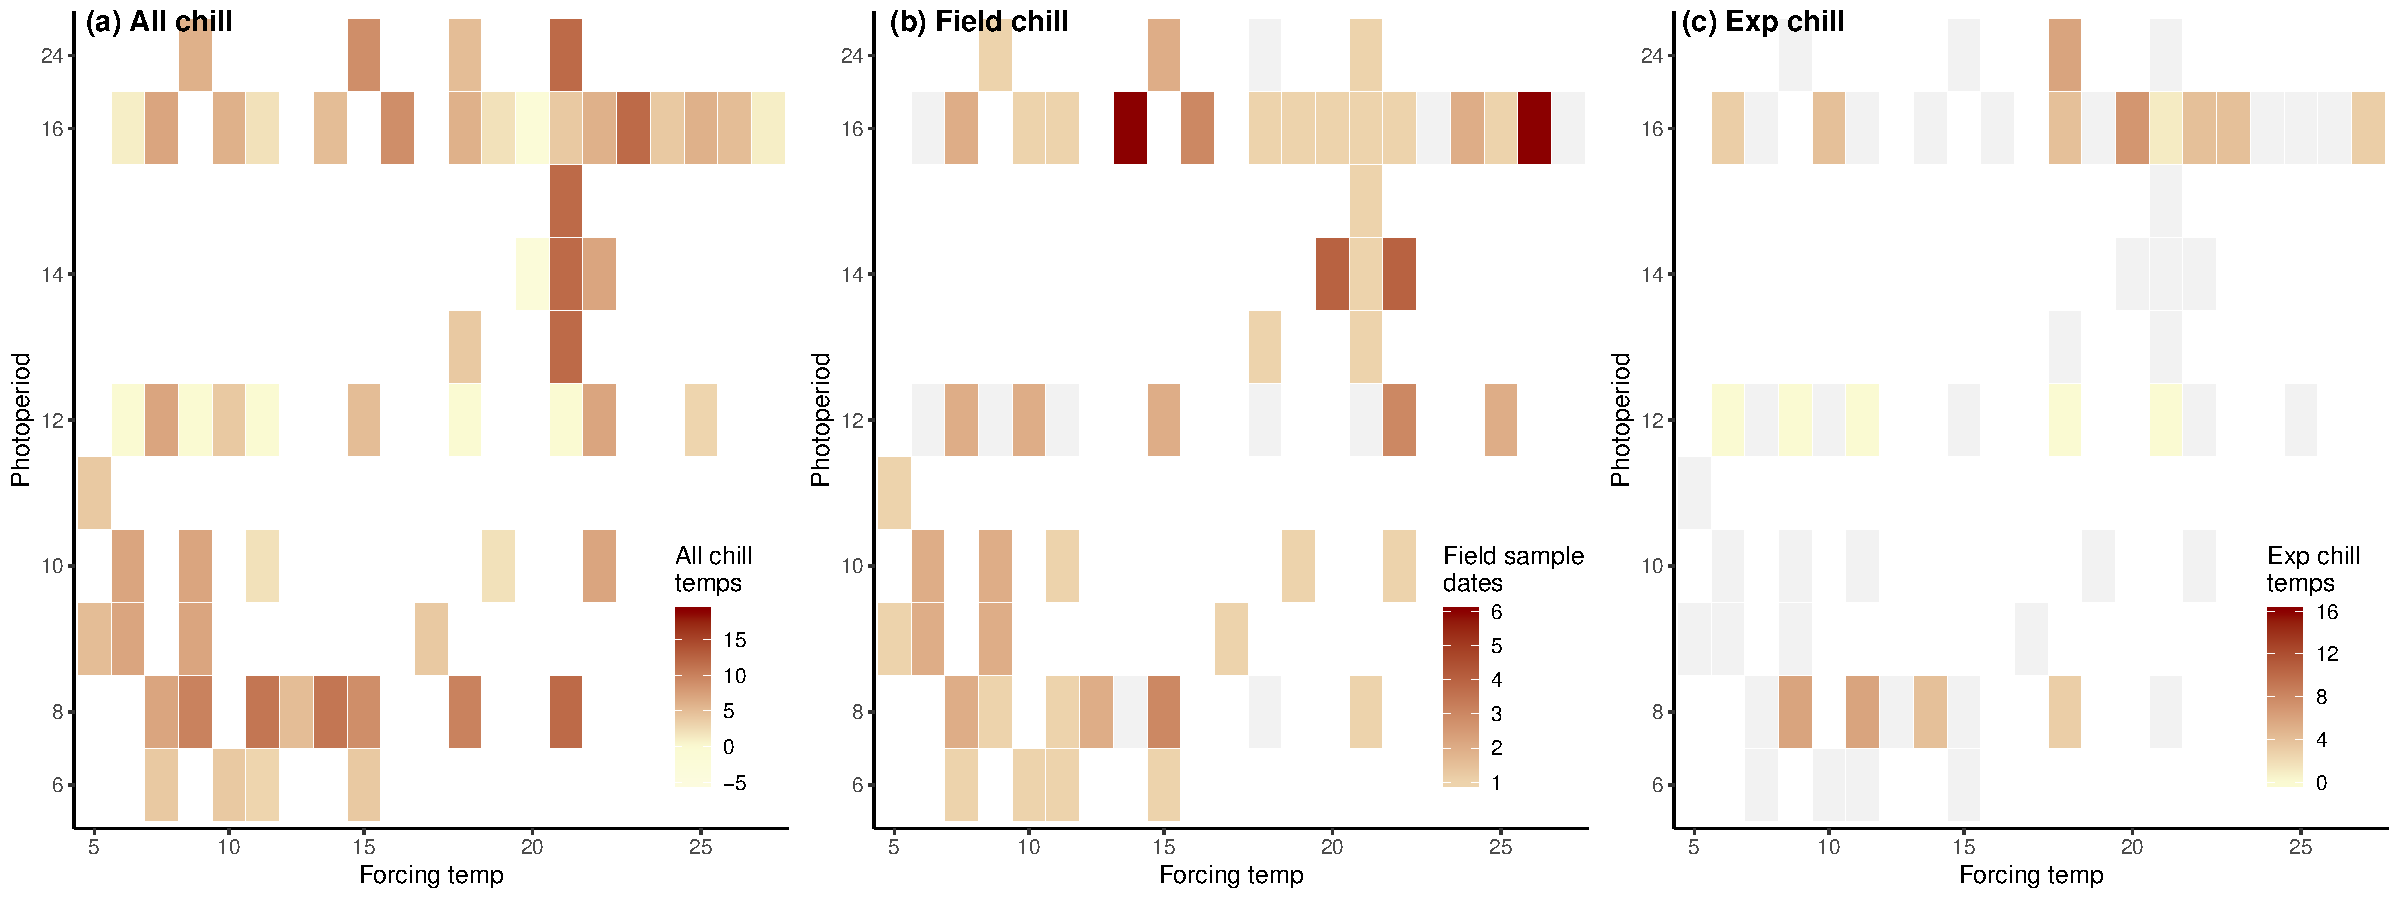
\includegraphics[width=0.9\textwidth]{..//..//analyses/bb_analysis/figures/studydesign/studydesign_heat3panelmainmodel.pdf}
\caption{\textbf{The diversity of study designs used in analyses.} Heatmaps show the range and commonness of different forcing (x-axis in all panels) by photoperiod (y-axis in all panels) combinations and with which chilling they were combined. In (A, top and bottom) we show our estimated chill units, which integrate across field (B, top and bottom) and experimental chilling (C, top and bottom). The top row shows all data included in the full model with 203 species, while the bottom row shows the data included in the main model with a subset of species well-represented across treatments and studies. Gray squares indicate a treatment was not applied (\emph{i.e.}, the prevalence of gray squares in (C) highlights how few studies include experimental chilling). Field sample dates are counted as any reported sampling dates more than 14 days apart.}
\label{fig:treatheatmaps}
\end{figure}


\begin{figure}[h!]
\centering
\noindent 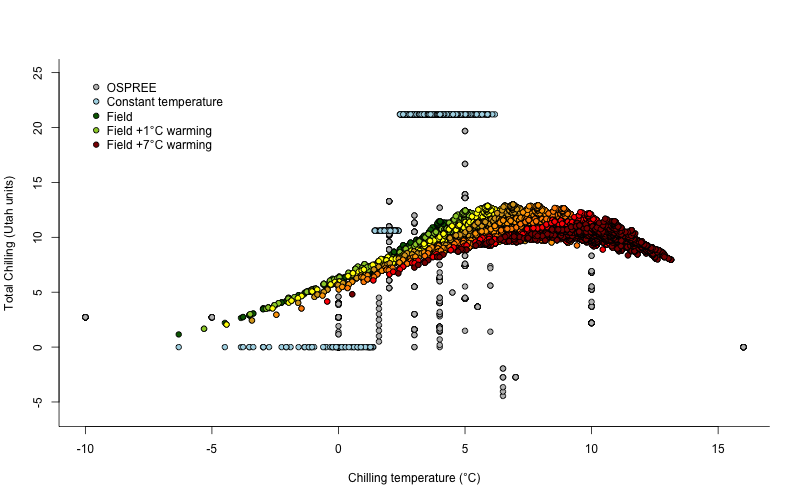
\includegraphics[width=0.50\textwidth]{..//..//analyses/bb_analysis/figures/EDFig4_exp_vs_field_chill_withwarmingcols.png}
\caption{\textbf{Chilling accumulates differently in experiments with constant temperatures versus natural systems}, in which temperature is more strongly correlated with chilling. See \emph{Estimating chilling} for a detailed description of ``Field'' climate data, for which we use historical climate data from Europe. Fig. \ref{fig:3dfieldchillutah} uses ``Field'' relationships (i.e., climate data and relationships from field chilling conditions to convert chill temperature to total chilling), whereas Fig. \ref{fig:3dexpchillutah} uses ``Constant temperature'' conditions (i.e., analagous to most experimental conditions) to estimate total chilling (see `Estimating chilling' in \emph{Methods} for details).}
\label{fig:chillexpfield}
\end{figure}

\begin{figure}[h!]
\centering
\noindent 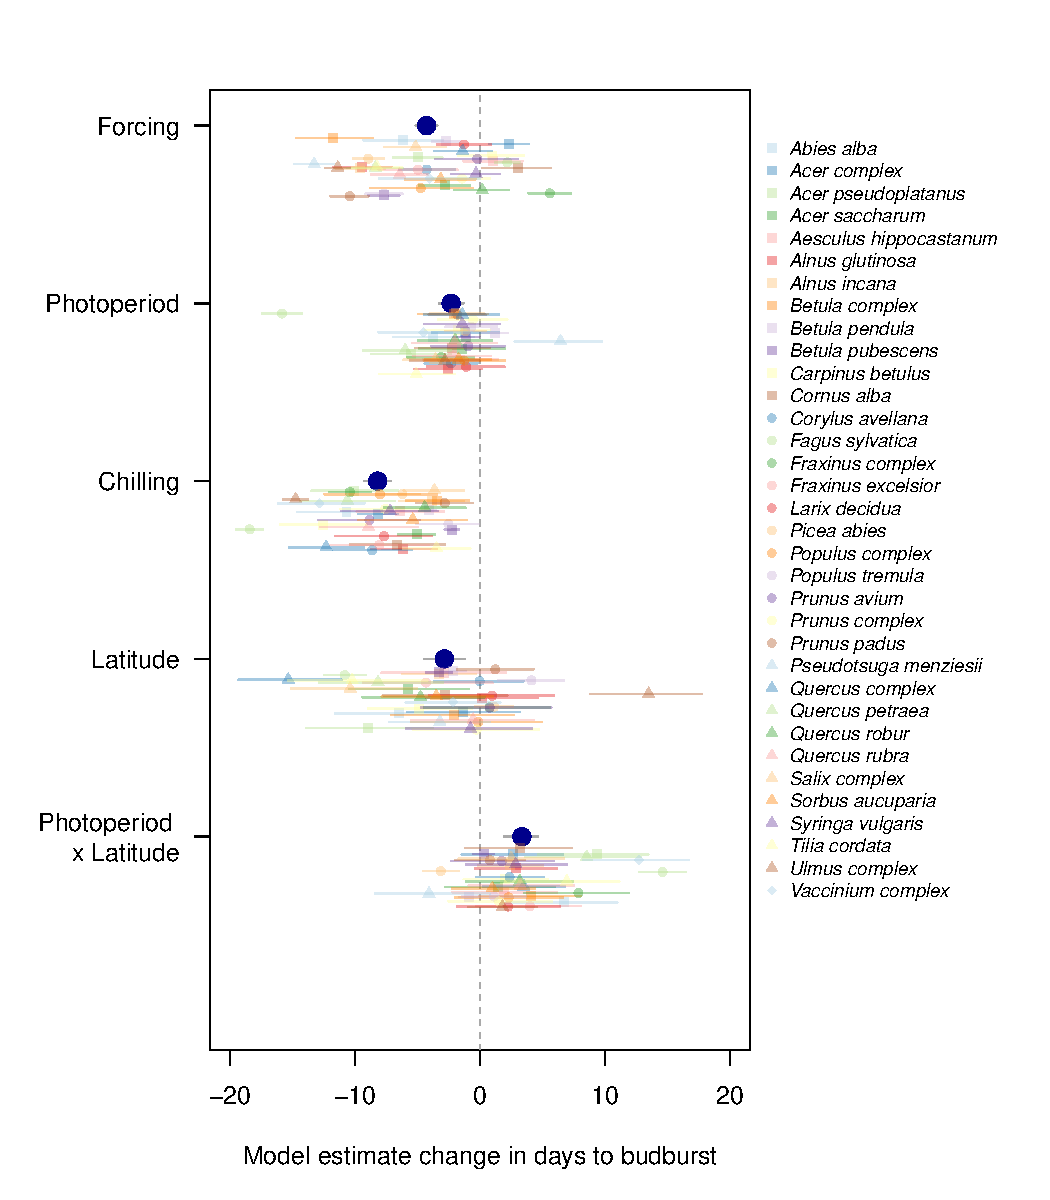
\includegraphics[width=0.75\textwidth]{..//..//analyses/lat_analysis/figures/EDFig5_latanalysis_spcom_expramp_fp.pdf}
\caption{\textbf{Estimates for effects of chilling exceeded estimates for forcing, photoperiod, provenance latitude, and the interaction between latitude and photoperiod, for most species,} in the latitude budburst model, using Utah units (Table \ref{tab:lat}). Using standardized units, which allow comparisons across cues, we show that, as with the main budburst model (Fig. \ref{fig:mu}), most species (smaller symbols) are responsive to most cues. Chilling is the strongest cue when considering overall estimates across species (larger, dark blue circles).}
\label{fig:lat}
\end{figure}


\begin{figure}[h!]
\centering
\noindent 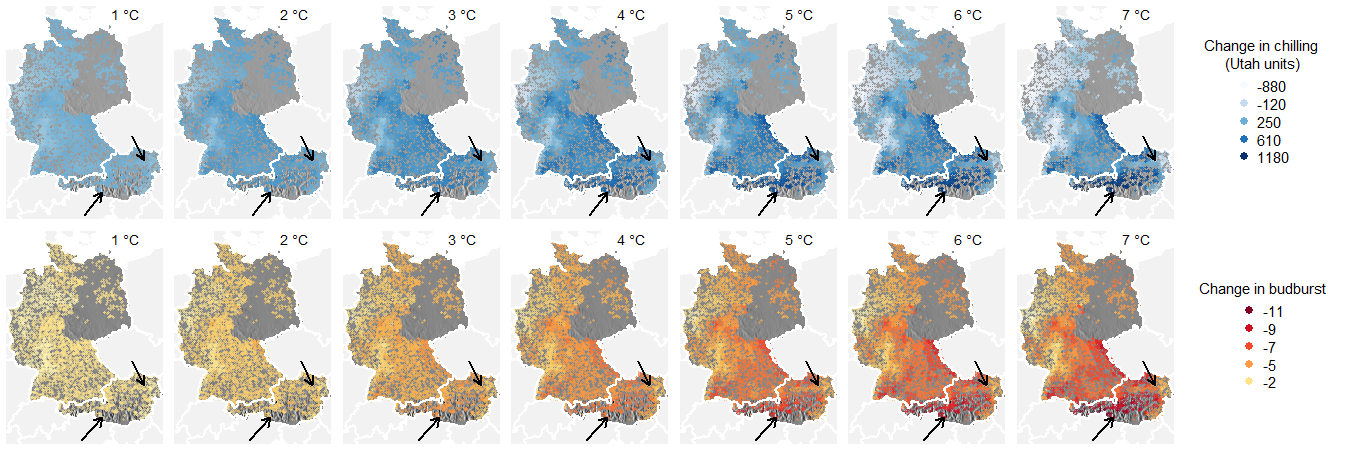
\includegraphics[width=0.90\textwidth]{..//..//analyses/bb_analysis/figures/forecasting/EDFig6_heatmapsbetpepfinalarrows.png}
\caption{\textbf{Forecasted changes in chilling and spring phenology vary with amount of warming across European locations included in the PEP725 database}. Changes in chilling (top panel) and budburst for \emph{Betula pendula} (bottom panel) are calculated relative to the mean chilling and leafout dates during a pre-warming time period (1951-1960) for each location. Arrows indicate sites shown in Figs. \ref{fig:betfag3d}A and \ref{fig:betfag2d}A (latitude = 46.8\degree N, longitude =  12.8\degree E, 659 m above sea level) and Figs. \ref{fig:betfag3d}B and \ref{fig:betfag2d}B (latitude = 48.3\degree N, longitude =  15.8\degree E, 210 m above sea level).} 
\label{fig:foremap}
\end{figure}

\begin{figure}[h!]
\centering
\noindent 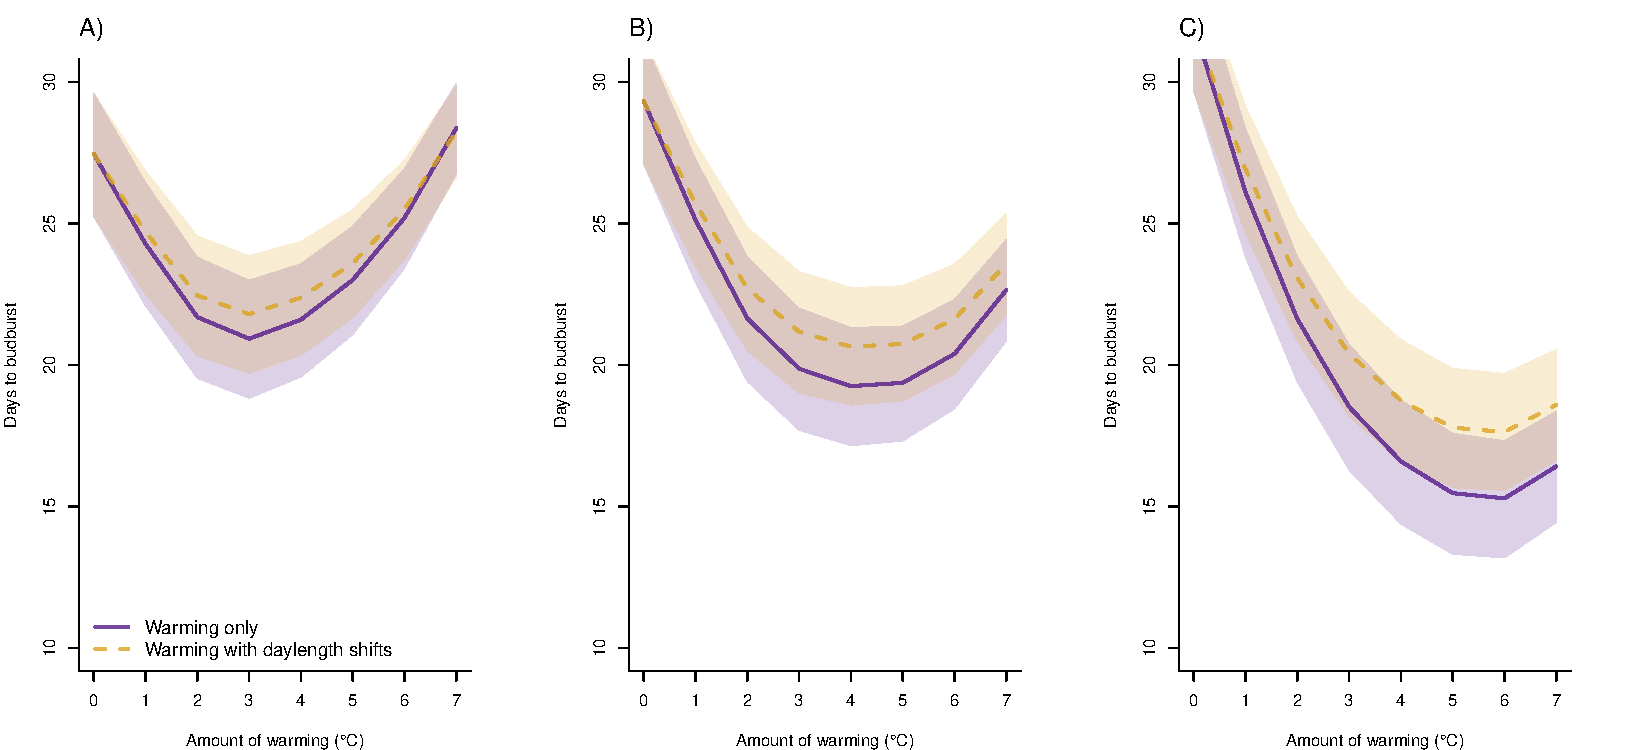
\includegraphics[width=0.75\textwidth]{..//..//analyses/bb_analysis/figures/forecasting/EDFig7_fagsyl_3lats.pdf}
\caption{\textbf{Budburst is affected by climate-change induced shifts in photoperiod, especially at high latitudes}, though effects vary by site and are minor compared to effects of warming. We show forecasted effects of varying levels of warming on \emph{Fagus sylvatica}, the most photoperiod-sensitive species in our database, across three latitudes within its range, as predicted by the latitude model. The low latitude site (A) is  located at 46.8\degree N, 15.7\degree E; the mid-latitude site (B) is located at 47.7\degree N, 16.3\degree E; and the high-latitude (C) site is located at 48.8\degree N, 15.4\degree E.}
\label{fig:fagsyllat}
\end{figure}

\newpage
\begin{figure}[h!]
\centering
\noindent 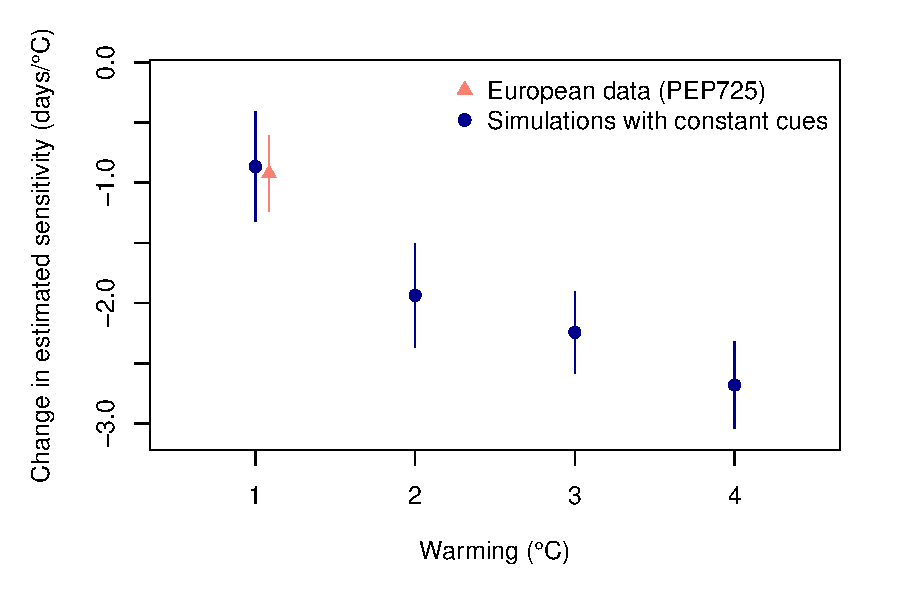
\includegraphics[width=0.75\textwidth]{..//..//analyses/bb_analysis/PEP_climate/figures/EDFig8_peprealandsims.pdf}
\caption{\textbf{Declining sensitivities observed in long-term European data for a suite of common trees may be explained by a statistical artifact.} We compared the sensitivity estimated from linear regressions of day of leafout versus mean spring temperature (estimated thus as days/$^{\circ}$C) from PEP725 data for \emph{Betula pendula} from 45 sites (``European data'') with estimated declines in simulations where the cues were held constant but spring temperatures warmed by 1-4$^{\circ}$C (``Simulations'') and found the estimated temperature sensitivity measured as days/$^{\circ}$C declined even though the underlying cues had not changed, see \emph{Potential statistical artifacts in declines of temperature sensitivity in observational long-term data} in the Supplemental Materials for further details.}
\label{fig:pepsims}
\end{figure}

\newpage
\begin{figure}[h!]
\centering
\noindent 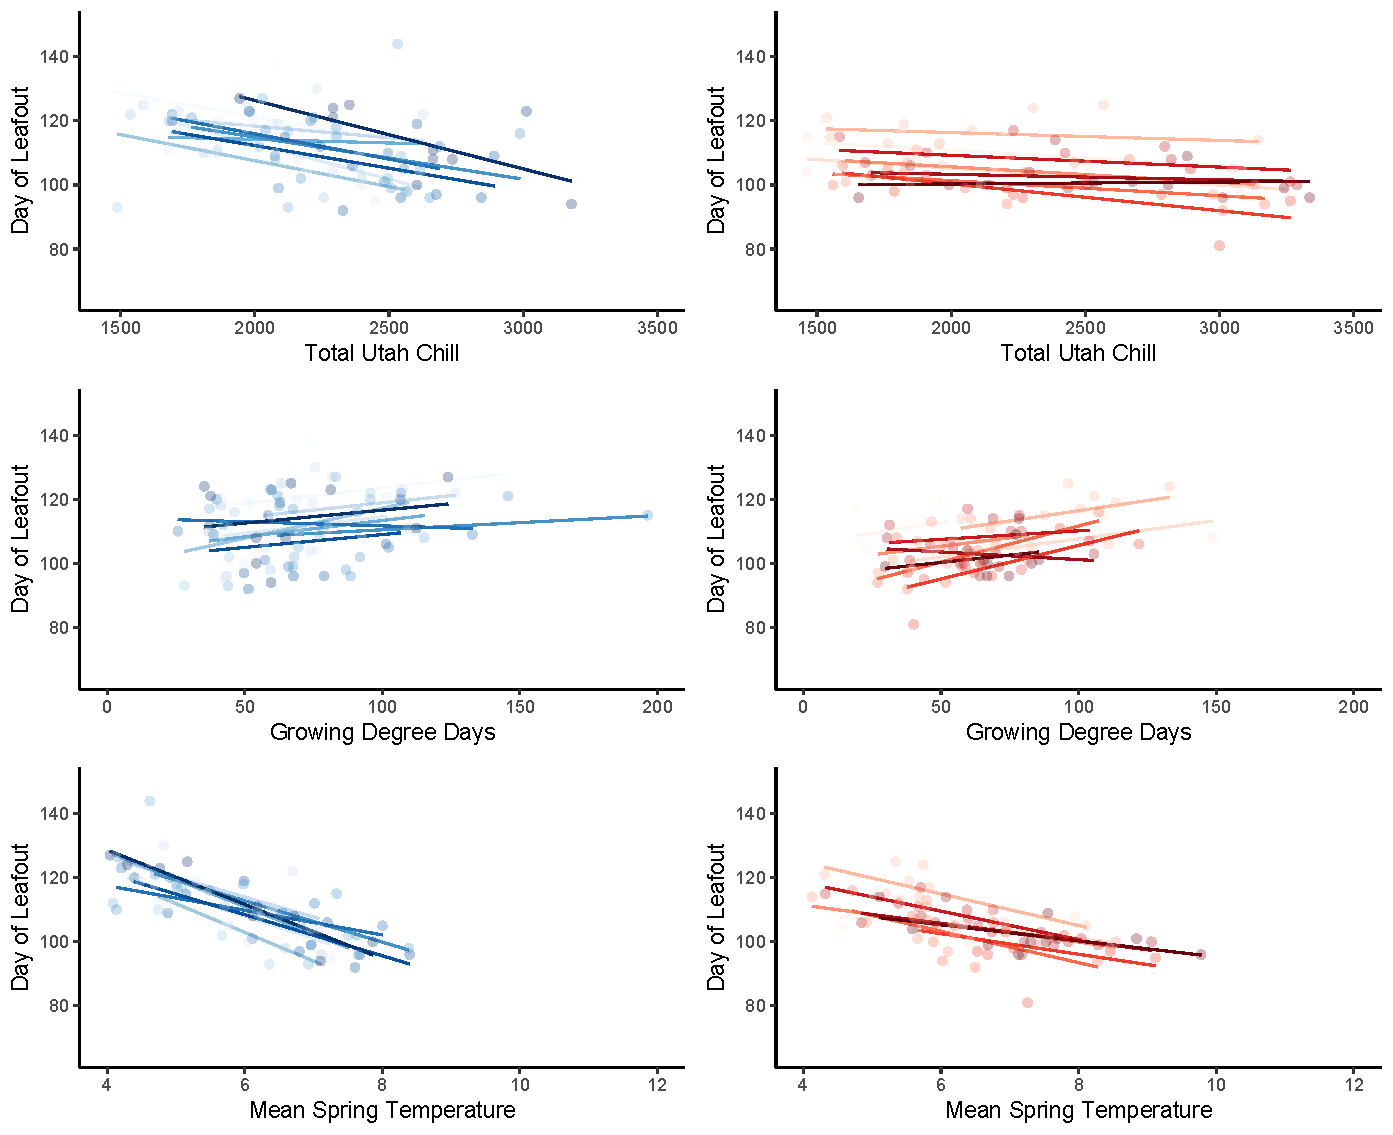
\includegraphics[width=0.75\textwidth]{..//..//analyses/bb_analysis/PEP_climate/figures/EDFig9_betpen_multruns_utahgddmat.pdf}
\caption{\textbf{Day of leafout varies with chilling, growing degree-days, and mean spring temperature.} These relationships are shown pre-warming (left panels, 1951-1960) and post-warming (right panels, 2000-2010) for PEP725 sites in Germany where \emph{Betula pendula} phenology has been monitored for decades.}
\label{fig:pep}
\end{figure}

\begin{figure}[h!]
\centering
\noindent 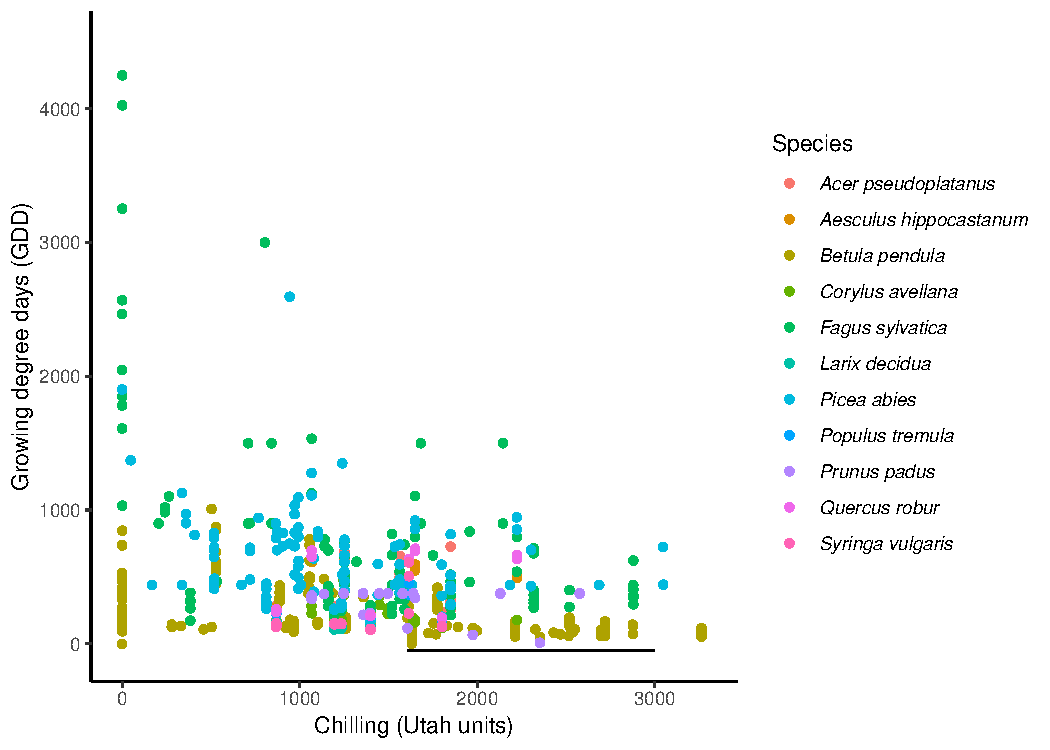
\includegraphics[width=1\textwidth]{..//..//analyses/bb_analysis/figures/EDFig10_gddbyutah_pepspp.pdf}
\caption{\textbf{Growing degree days (GDD) versus chill units at the time of budburst} from the OSPREE database for common species in the PEP725 long-term phenological database. The black line shows the range of chilling (10-90\% quantiles) accumulated from 1 September to 1 March for 45 sites for \emph{Betula pendula} (see also \emph{Potential statistical artifacts in declines of temperature sensitivity in observational long-term data} in the Supplemental Materials). We calculated GDD here as the average daily forcing temperature multiplied by days to budburst.}
\label{fig:pepgddchill}
\end{figure}

%%%%%%%%%%%%%%%%%%%%%%%%%%%%%%%%%%%%%%%%
\end{document}
%%%%%%%%%%%%%%%%%%%%%%%%%%%%%%%%%%%%%%%%
